\documentclass{article}
\usepackage{pgfplots}\pgfplotsset{compat=1.18}
\begin{document}
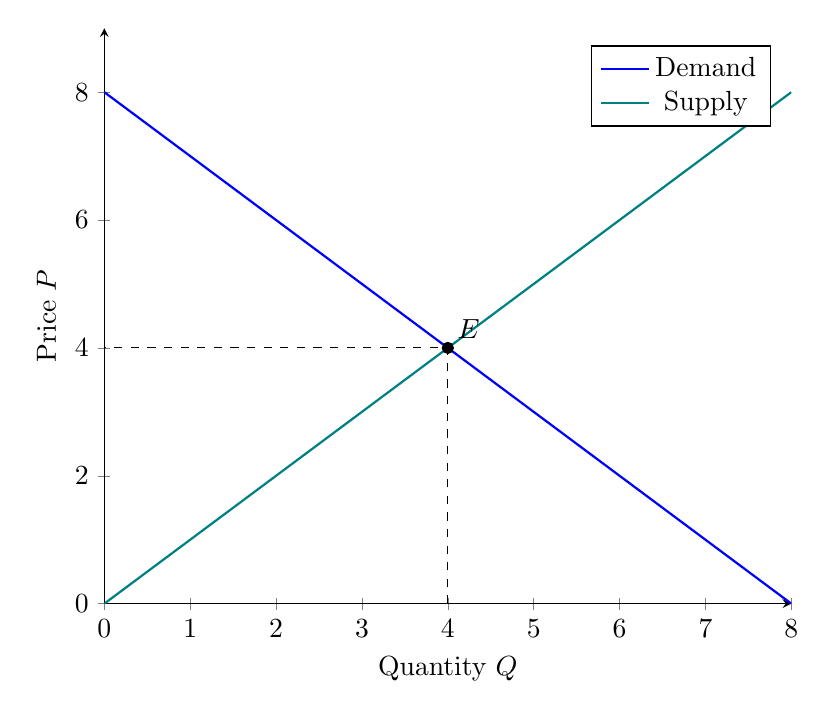
\begin{tikzpicture}
\begin{axis}[width=.85\linewidth,xmin=0,xmax=8,ymin=0,ymax=9,
xlabel={Quantity $Q$},ylabel={Price $P$},axis lines=left,legend pos=north east]
\addplot[blue,thick,domain=0:8]{8-x};\addlegendentry{Demand}
\addplot[teal,thick,domain=0:8]{x};\addlegendentry{Supply}
\addplot[only marks,mark=*,black] coordinates {(4,4)};
\draw[dashed] (axis cs:4,0)--(axis cs:4,4)--(axis cs:0,4);
\node[above right] at (axis cs:4,4){$E$};
\end{axis}\end{tikzpicture}
\end{document}
